%%
%% This is file `sample-sigconf.tex',
%% generated with the docstrip utility.
%%
%% The original source files were:
%%
%% samples.dtx  (with options: `sigconf')
%% 
%% IMPORTANT NOTICE:
%% 
%% For the copyright see the source file.
%% 
%% Any modified versions of this file must be renamed
%% with new filenames distinct from sample-sigconf.tex.
%% 
%% For distribution of the original source see the terms
%% for copying and modification in the file samples.dtx.
%% 
%% This generated file may be distributed as long as the
%% original source files, as listed above, are part of the
%% same distribution. (The sources need not necessarily be
%% in the same archive or directory.)
%%
%%
%% Commands for TeXCount
%TC:macro \cite [option:text,text]
%TC:macro \citep [option:text,text]
%TC:macro \citet [option:text,text]
%TC:envir table 0 1
%TC:envir table* 0 1
%TC:envir tabular [ignore] word
%TC:envir displaymath 0 word
%TC:envir math 0 word
%TC:envir comment 0 0
%%
%%
%% The first command in your LaTeX source must be the \documentclass command.
\documentclass[sigconf]{acmart}

\renewcommand\footnotetextcopyrightpermission[1]{} % removes conference footnote
\settopmatter{printacmref=false}
\settopmatter{printccs=false}     % Removes CCS concepts section
\settopmatter{printfolios=false}  % Removes page numbers (optional)

\fancyhead{}  % clear all header fields

%%
%% \BibTeX command to typeset BibTeX logo in the docs
\AtBeginDocument{%
  \providecommand\BibTeX{{%
    \normalfont B\kern-0.5em{\scshape i\kern-0.25em b}\kern-0.8em\TeX}}}

\usepackage{algorithm} 
\usepackage{algpseudocode} 
\usepackage{makecell} 
\usepackage{xspace} 
\usepackage[nocomma]{optidef}
% don't add package ulem, otherwise bib will be underlined
% \usepackage{ulem} 
\usepackage{enumitem}
\usepackage{graphicx}
\usepackage{subcaption}
\usepackage{multirow}
\usepackage{balance}

%%
%% end of the preamble, start of the body of the document source.
\acmBooktitle{Numerical Analysis for Machine Learning Project 2024-2025}
\begin{document}

%%
%% The "title" command has an optional parameter,
%% allowing the author to define a "short title" to be used in page headers.
\title[Combining Autoencoders and Deep Learning for Effective Fraud Detection in Credit Card Transactions]{Combining Autoencoders and Deep Learning for Effective Fraud Detection in Credit Card Transactions}

% \author{Beatrice Zani, Niccolò Salvi}
% \email{beatrice.zani@mail.polimi.it, niccolo1.salvi@mail.polimi.it}

\author{Beatrice Zani}
\email{beatrice.zani@mail.polimi.it}
\affiliation{
  \institution{Politecnico di Milano}
  \department{Dipartimento di Elettronica, Informazione e Bioingegneria}
  \city{Milan}
  \country{Italy}
}

\author{Niccolò Salvi}
\email{niccolo1.salvi@mail.polimi.it}
\affiliation{
  \institution{Politecnico di Milano}
  \department{Dipartimento di Elettronica, Informazione e Bioingegneria}
  \city{Milan}
  \country{Italy}
}

%%
%% The abstract is a short summary of the work to be presented in the
%% article.
\begin{abstract}
Credit card fraud detection presents significant challenges due to the extreme imbalance between fraudulent and legitimate transactions. This study implements and evaluates an advanced fraud detection framework combining autoencoders, attention-based Long Short-Term Memory networks (ALSTM), and gradient boosting techniques. First, an autoencoder trained exclusively on fraudulent transactions captures their underlying data distribution. Subsequently, synthetic fraudulent samples generated by the autoencoder are filtered using a Support Vector Machine (SVM) to improve realism and data balance. Finally, an ALSTM model wrapped within a gradient boosting framework effectively classifies transactions by leveraging temporal dependencies and attention mechanisms. Results demonstrate enhanced detection performance, achieving high discriminative power with minimal false positives. This approach significantly improves upon traditional methods, providing robust solutions in handling extreme class imbalances inherent in fraud detection problems.
\end{abstract}

%%
%% Keywords. The author(s) should pick words that accurately describe
%% the work being presented. Separate the keywords with commas.
\keywords{Credit Card Fraud Detection, Autoencoder, Attention-based LSTM, Gradient Boosting, Class Imbalance, Anomaly Detection}

%% information and builds the first part of the formatted document.
\maketitle

\section{Introduction}

In today's evolving digital economy, credit card fraud poses significant challenges for financial institutions and customers alike. According to the European Banking Authority (EBA) and the European Central Bank (ECB) report on Fraud Payments\footnote{2024 REPORT ON PAYMENT FRAUD, \url{https://www.ecb.europa.eu/press/intro/publications/pdf/ecb.ebaecb202408.en.pdf}}, fraudulent card-based transactions amounted to EUR 4.3 billion in 2022 and EUR 2.0 billion in the first half of 2023. Increasing transaction volumes, evolving fraudulent methods, and the inherent rarity of fraud incidents compared to legitimate transactions complicate detection efforts. Consequently, there is a growing reliance on machine learning methods to swiftly and accurately detect suspicious activities.

Fundamentally, fraud detection is framed as a binary classification task, distinguishing fraudulent from legitimate transactions by identifying anomalous patterns in data. This research leverages advanced machine learning techniques—autoencoders, attention-based long short-term memory (ALSTM) networks, gradient boosting (GB), and support vector machines (SVM)—to capture nuanced and complex transaction behaviors. Specifically, we replicate and extend the approach introduced by Mohammed Tayebi and Said El Kafhali in their paper \textbf{Combining Autoencoders and Deep Learning for Effective Fraud Detection in Credit Card Transactions}\cite{Tayebi2025}.

Autoencoders offer robust performance by learning latent representations of data, making them particularly suited for anomaly detection. Additionally, ALSTM networks excel at identifying significant temporal patterns within sequential transaction data through attention mechanisms. Building upon these techniques, we propose a comprehensive framework where an autoencoder initially models the fraud transaction distribution, generates synthetic fraud samples, and refines them via an SVM-based filtering strategy. Subsequently, these refined datasets feed into an ALSTM network integrated within a gradient boosting ensemble to enhance detection capabilities.

The contributions of this paper include: (i) developing a specialized pipeline tailored for severely imbalanced fraud detection scenarios; (ii) improving synthetic data realism through an SVM-filtered autoencoder strategy; and (iii) validating superior performance over conventional machine learning and basic deep learning methods.
\section{Background and Reproduction Objectives}

Credit card fraud detection has traditionally relied upon supervised machine learning techniques such as logistic regression, decision trees, and classical ensemble methods (e.g., random forests and gradient boosting). However, the inherent data imbalance in fraud detection datasets severely limits these traditional methods, resulting in low precision and a high rate of false positives.

Recent advances in deep learning offer promising solutions. Particularly, autoencoders have emerged as powerful tools due to their ability to learn effective representations of transaction data, thus providing an unsupervised or semi-supervised approach to fraud detection. Additionally, Long Short-Term Memory (LSTM) networks, especially those augmented with attention mechanisms (ALSTM), have proven effective in modeling sequential transaction data by dynamically emphasizing informative temporal patterns.

The core objective of this project is to replicate and evaluate the effectiveness of an existing methodology integrating these techniques, specifically autoencoders, ALSTM, and gradient boosting frameworks, as presented in prior research. In replicating this approach, we aim to validate its efficacy on widely-used benchmark datasets, confirm its robustness to severe class imbalance, and identify potential areas for improvement or optimization in both training procedures and model architectures.

To achieve these objectives, the project systematically follows the established approach: an autoencoder is trained solely on fraudulent samples to learn their distinctive features and generate realistic synthetic fraud data. These generated samples undergo a further refinement step using a Support Vector Machine (SVM) to eliminate unrealistic or unrepresentative synthetic examples, thereby enhancing the training set quality. Subsequently, the cleaned, balanced dataset is employed to train an ALSTM-based classification model wrapped within a gradient boosting ensemble to achieve optimal predictive performance.

Through this structured replication, we also explore the impact of model hyperparameters, regularization techniques, and training strategies on model performance, seeking to provide clear, reproducible guidelines and insights that contribute toward advancing research in anomaly and fraud detection.

\section{Theoretical Background}
This section introduces the core machine learning techniques used in our fraud detection framework. Each method was selected for its specific strengths in addressing the challenges posed by imbalanced datasets, temporal dependencies, and anomaly detection. We provide a concise overview of Autoencoders, Support Vector Machines (SVM), Recurrent Neural Networks (RNN) and Long Short-Term Memory (LSTM) architectures with attention mechanisms, and Gradient Boosting, highlighting their relevance and applicability to our problem.

\subsection{Autoencoders}
Autoencoders\cite{Rumelhart1986LearningRB} are a class of neural networks designed to learn efficient codings of input data in an unsupervised manner. They consist of two main components: an encoder, which compresses the input into a lower-dimensional latent representation, and a decoder, which reconstructs the input from this latent space. The network is trained to minimize the difference between the original input and its reconstruction, effectively learning to capture the most salient features of the data. Autoencoders are particularly useful in anomaly detection tasks, where the model is trained on normal data and expected to perform poorly on anomalous inputs that deviate from the learned patterns.

\subsection{SVM}
Support Vector Machines (SVMs)\cite{10.1023/A:1022627411411} are supervised learning models used for classification and regression tasks. They operate by finding the optimal hyperplane that separates data points of different classes with the maximum margin (distance of closest point to the boundary). In high-dimensional spaces, or when data is not linearly separable, SVMs utilize kernel functions to map inputs into higher-dimensional feature spaces where a linear separator may exist. SVMs are valued for their robustness and effectiveness in dealing with small to medium-sized datasets, especially in cases where class boundaries are well-defined.

\subsection{ALSTM}
\subsubsection{Recurrent Neural Networks}
Traditional neural networks typically assume inputs are independent and identically distributed, neglecting temporal or sequential dependencies among data points. However, in real-world tasks such as credit card fraud detection, transactions often exhibit meaningful sequential patterns and contextual relationships that are essential for accurate classification.

Recurrent Neural Networks (RNNs)\cite{rumelhart1985learning} are explicitly designed to address this limitation by incorporating internal states or memories, allowing the network to retain information from previous inputs. Unlike feedforward neural networks, RNNs maintain and update hidden states using recurrent connections, enabling them to effectively capture temporal dependencies within sequential data. Consequently, RNNs are well-suited for modeling transaction sequences and identifying complex, evolving fraud patterns.

\subsubsection{Long Short-Term Memory Networks (LSTM)}
Long Short-Term Memory (LSTM)\cite{6795963} networks were specifically developed to overcome the limitations of standard RNNs. The key advantage of LSTMs is their ability to retain relevant context over extended periods, making them particularly effective for capturing long-term sequential dependencies.

An LSTM network achieves this through specialized gating mechanisms that control the flow of information within the network's hidden states. Each LSTM cell comprises three primary gates:

\begin{itemize}
    \item \textbf{Forget Gate}: Determines which information from previous hidden states should be discarded.
    \item \textbf{Input Gate}: Decides which new information should be stored in the hidden state.
    \item \textbf{Output Gate}: Controls what part of the hidden state should be exposed at the output.
\end{itemize}

Collectively, these gates enable the LSTM to manage memory selectively, preserving essential information across longer sequences and discarding irrelevant or outdated context, thereby overcoming the vanishing gradient issue inherent in standard RNNs.

\subsubsection{Attention Mechanisms}
While LSTMs significantly enhance the capability to capture long-term dependencies, they still process sequences linearly, giving equal implicit attention to all elements in a sequence. Attention mechanisms were introduced to overcome this limitation by dynamically assigning weights to different elements within a sequence based on their relevance to the task at hand~\cite{bahdanau2016neuralmachinetranslationjointly}.

Specifically, the attention mechanism computes a context vector as a weighted sum of the hidden states produced by the LSTM network. The weights assigned to each hidden state reflect the importance of each transaction within the sequence. This selective focus enables the model to effectively highlight significant events, drastically improving performance on tasks such as fraud detection, where identifying the critical anomalous patterns within sequences is essential.

Formally, given hidden states \(h_1, h_2, \dots, h_n\), the attention mechanism computes weights \(a_{ij}\) using:

\[
a_{ij} = \frac{\exp(\alpha(s_{i-1}, h_j))}{\sum_{k=1}^{n}\exp(\alpha(s_{i-1}, h_k))}
\]

where \(\alpha(s_{i-1}, h_j)\) is an alignment function measuring compatibility between the hidden state \(h_j\) and the previous decoder state \(s_{i-1}\). The context vector \(C_i\) is then computed as:

\[
C_i = \sum_{j=1}^{n} a_{ij}h_j
\]

Through this focused selection of relevant transaction information, attention-based LSTM networks significantly enhance fraud detection performance by capturing critical sequential patterns more effectively than traditional methods.

\subsection{Gradient Boosting}
Gradient Boosting\cite{4a848dd1-54e3-3c3c-83c3-04977ded2e71} is a powerful ensemble learning technique used primarily for classification and regression tasks.
Unlike bagging methods, which train multiple models in parallel and combine their outputs, boosting builds an ensemble sequentially, where each new model attempts to correct the errors of its predecessors. Boosting aims at reducing bias without increasing variance to obtain a more powerful learner. 

The core idea behind gradient boosting is to train a sequence of weak learners—typically decision trees—where each learner focuses on minimizing the residual errors made by the combined ensemble so far. The process begins by fitting a model to the data and computing the loss (e.g., classification error). The next model is then trained to predict the gradient of the loss function with respect to the predictions, effectively reducing the overall error step by step.

Formally, given a loss function $L(y, \hat{y})$ and a model $F_m(x)$ at iteration $m$, gradient boosting updates the model as:

\[
F_{m+1}(x) = F_m(x) + \gamma_m h_m(x)
\]

where $h_m(x)$ is a new weak learner trained to approximate the negative gradient of the loss with respect to $F_m(x)$, and $\gamma_m$ is a step size (also known as the learning rate).

This iterative approach enables gradient boosting to build highly accurate models by combining the strengths of many simple learners. Moreover, the method can be adapted to support a variety of base learners beyond decision trees, such as neural networks, which allows integration with deep learning architectures.

Gradient boosting is especially useful in imbalanced classification problems, as it can adaptively focus more on difficult or rare instances—such as fraudulent transactions—by increasing their influence in subsequent iterations. When combined with models like attention-based LSTMs, gradient boosting provides a robust framework capable of learning complex data patterns while reducing overfitting.
\section{Methodology}
This section outlines the implementation pipeline developed for replicating and extending the referenced fraud detection framework. We begin by preprocessing the dataset and training an autoencoder exclusively on fraudulent transactions to learn their underlying distribution. This autoencoder is then used to generate synthetic fraudulent samples, which are subsequently filtered using a Support Vector Machine (SVM) to ensure data quality. The resulting dataset is used to train an attention-based Long Short-Term Memory (ALSTM) network integrated into a gradient boosting ensemble for final classification. Each stage of the pipeline is detailed in the subsections that follow.

\subsection{Dataset Analysis and Preprocess}
The dataset employed in this project is the widely used \texttt{Credit Card Fraud Detection dataset}, made publicly available by \textit{Worldline and the Machine Learning Group at Université Libre de Bruxelles (ULB)}. The dataset is accessible for download from the \textit{Credit Card Fraud Detection}'s Kaggle repository\footnote{\url{https://www.kaggle.com/datasets/mlg-ulb/creditcardfraud}}.

This dataset contains transactions made by European cardholders over a period of two days in September 2013, comprising a total of 284,807 transactions, among which only 492 are labeled as fraudulent. This severe class imbalance (fraudulent transactions represent just 0.172\% of the total), as seen in Figure~\ref{fig:class-distribution}, makes it a challenging benchmark for anomaly detection and imbalanced classification tasks and motivates the use of specialized techniques such as synthetic data generation and class balancing strategies, which are detailed in subsequent sections.

Each transaction in the dataset is described by a total of 31 numerical features:
\begin{itemize}
    \item 28 features are anonymized principal components resulting from a \texttt{PCA} (Principal Component Analysis) transformation applied to the original dataset to preserve confidentiality (labeled from \texttt{V1} to \texttt{V28}).
    \item The remaining 3 features are:
        \begin{itemize}
            \item \texttt{Time}: The elapsed time (in seconds) from the first transaction in the dataset.
            \item \texttt{Amount}: The monetary amount of the transaction.
            \item \texttt{Class}: The target variable, where \texttt{1} indicates a fraudulent transaction and \texttt{0} indicates a legitimate one.
        \end{itemize}
\end{itemize}

\begin{figure}[h]
    \centering
    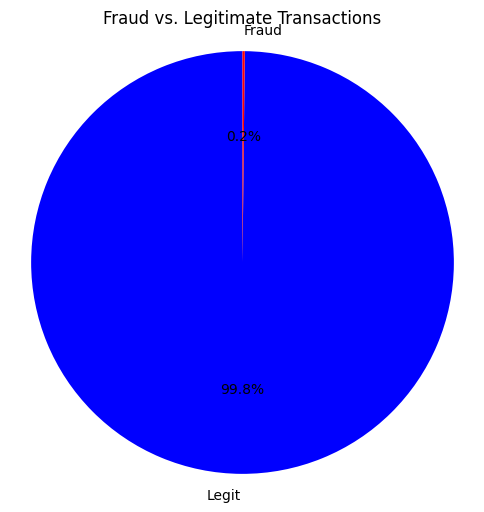
\includegraphics[width=0.25\textwidth]{images/fraud_vs_legit_pie.png}
    \caption{Distribution of Fraudulent vs. Legitimate Transactions}
    \label{fig:class-distribution}
\end{figure}

\subsubsection{Dataset Preprocess}
The dataset was preprocessed by removing the \texttt{Time} and \texttt{Label} columns. The \texttt{Time} feature was excluded based on recommendations from the original paper, as it did not significantly contribute to the learning process.

As suggested in the reference paper, the \texttt{Amount} feature was standardized using the \texttt{RobustScaler} transformation to reduce the influence of outliers, which are particularly common in financial transaction data.

\subsection{Autoencoder-based Fraud Pattern Modeling}
In our approach, we utilized an autoencoder neural network trained exclusively on fraudulent transactions to learn their internal structure and statistical properties. By exposing the model only to examples of fraud, we ensured its ability to specialize in recognizing the underlying data distribution of abnormal behaviors. This setup enables the model to generate new, synthetic fraud samples that maintain the intrinsic characteristics of real fraud cases.

To enhance the model’s generalization ability, we split the fraudulent samples into training and validation subsets. The reconstruction performance on the validation set guided model tuning and early stopping to prevent overfitting.

The autoencoder architecture is symmetric, with an encoder compressing the 29 input features through successive layers, and a decoder reconstructing the input by reversing the encoding path. Dropout regularization was employed in both parts of the network to combat overfitting by randomly deactivating a subset of neurons during training. Table~\ref{tab:autoencoder_architecture} summarizes the layer configuration of both encoder and decoder components.

The model was trained to minimize the reconstruction loss between the input $x$ and the output $\hat{x}$ using the Mean Squared Error (MSE) loss function:
\[
J(w, \hat{w}) = \frac{1}{n} \sum_{i=1}^{n} \frac{1}{2} \| x_i - \hat{x}_i \|^2
\]
Additionally, $L1$ regularization was applied to the network parameters to promote sparsity in the weights and reduce overfitting. The total loss function is a combination of MSE and the $L1$ norm:
\[
\mathcal{L}_{\text{total}} = \text{MSE} + \lambda \sum_{j} |w_j|
\]
where $\lambda$ is a regularization coefficient empirically set to $1 \times 10^{-3}$.

The model was trained using the \texttt{Adam} optimizer with an initial learning rate of $2 \times 10^{-4}$. A cosine annealing learning rate scheduler gradually reduced the learning rate over epochs, and early stopping was triggered if the validation loss did not improve for 75 consecutive epochs.

Once trained, the autoencoder was used to generate synthetic fraud samples by sampling latent representations and decoding them into realistic transaction vectors. These synthetic samples were later evaluated and filtered using a Support Vector Machine, as described in the following section.

\begin{table}[htbp]
    \small % or \scriptsize for even smaller
    \centering
    \begin{tabular}{|p{3.5cm}|p{3.5cm}|}
        \hline
        \textbf{Encoder} & \textbf{Decoder} \\
        \hline
        29 features (input) & 8 neurons, fully connected \\
        \hline
        23 neurons, fully connected & 17 neurons, fully connected \\
        \hline
        Dropout = 0.1 & Dropout = 0.2 \\
        \hline
        19 neurons, fully connected & 19 neurons, fully connected \\
        \hline
        Dropout = 0.2 & Dropout = 0.1 \\
        \hline
        17 neurons, fully connected & 23 neurons, fully connected \\
        \hline
        8 neurons, fully connected & 29 neurons, fully connected (output) \\
        \hline
    \end{tabular}
    \caption{Autoencoder architecture used for fraud modeling}
    \label{tab:autoencoder_architecture}
\end{table}

To monitor the learning progress of the autoencoder and ensure it generalizes well to unseen fraudulent samples, we plotted the training and validation loss across epochs. As shown in Figure~\ref{fig:autoencoder-loss}, the loss curves illustrate the convergence behavior of the model. The validation loss remains close to the training loss, indicating that the model is not overfitting and is effectively capturing the underlying patterns in fraudulent transactions.

\begin{figure}[h]
    \centering
    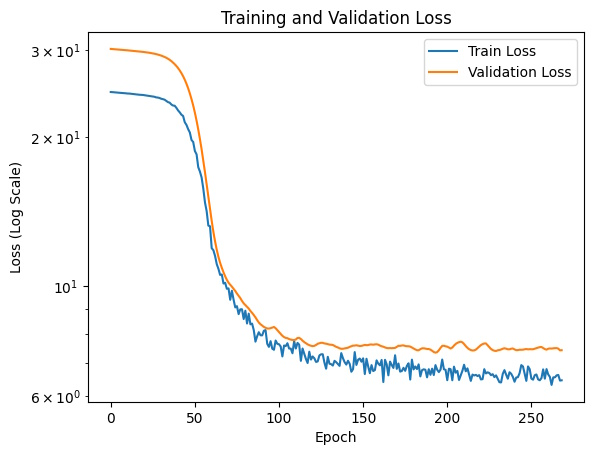
\includegraphics[width=0.45\textwidth]{images/autoencoder_loss.jpg}
    \caption{Training and validation loss of the autoencoder over epochs. The close alignment between the two curves indicates good generalization and absence of overfitting during training.}
    \label{fig:autoencoder-loss}
\end{figure}

\subsection{SVM Filtering of Synthetic Fraud Samples}
To improve the quality and realism of synthetic fraud data generated by the autoencoder, we introduced a filtering step using a Support Vector Machine (SVM). The goal of this step was to discard unrealistic or noisy synthetic examples that could degrade the training process of the subsequent classifier.

To train the SVM, a balanced dataset was constructed by randomly sampling an equal number of legitimate transactions to match the available genuine fraud samples. The two subsets were combined and assigned binary class labels, ensuring the SVM would learn a robust decision boundary between real fraud and legitimate data.

The combined dataset was shuffled and split into training and testing sets to evaluate generalization performance. A linear kernel was used for the SVM, prioritizing simplicity and interpretability. After training, the model achieved a training accuracy of \texttt{0.9438} and a testing accuracy of \texttt{0.9650}, indicating strong discriminative power on unseen samples.

Once trained, the SVM was applied to the synthetic samples generated by the autoencoder. Only those samples classified as fraudulent by the SVM were retained for the final training set. This filtering step significantly reduced the presence of unrealistic or misrepresentative samples, resulting in a cleaner, more trustworthy dataset for downstream classification.

After applying the SVM, only the synthetic samples classified as fraudulent were retained. This resulted in a final training set composed of \texttt{199008} legitimate and \texttt{199008} fraud samples, totalling \texttt{398016} samples used to train the ALSTM classifier.

\subsection{Attention-based LSTM Classifier}
To effectively detect fraudulent transactions in a sequential context, we employed an Attention-based Long Short-Term Memory (ALSTM) network as our final classification model. This choice is motivated by the observation that transaction sequences often contain temporal dependencies and behavioral patterns that are highly indicative of fraud.

\subsubsection{Motivation for Using ALSTM in Fraud Detection}
Fraudulent behavior frequently unfolds as a sequence of anomalies rather than isolated events. For example, fraudulent activity may be preceded by low-value "testing" transactions, rapid location changes, or abrupt deviations from typical purchasing behavior. Traditional feedforward networks lack the ability to capture these time-dependent patterns. ALSTM networks, by contrast, are well-suited for this task: the LSTM component models long-term dependencies across sequences, while the attention mechanism dynamically emphasizes the most relevant time steps for making predictions. This dual capability allows the model to prioritize significant contextual information during classification.

\subsubsection{Data Preparation and Input Format}
After generating a balanced dataset through synthetic fraud generation and SVM-based filtering, we reshaped the data to fit the expected input of the ALSTM network. Each sample was treated as a univariate sequence with a fixed length of 1 (since each transaction is an independent vector of features, not a true multistep temporal sequence).

\subsubsection{Model Architecture and Training}
The ALSTM architecture implemented in this project consists of the following components:
\begin{itemize}
    \item Two stacked LSTM layers, each with 50 hidden units, processing the transaction feature vectors. Both LSTM layers employed dropout regularization with a dropout rate of 0.3 and a recurrent dropout of 0.2 to prevent overfitting.
    \item A custom attention mechanism applied over the outputs of the second LSTM layer, dynamically weighting each time step's output to create a focused context vector.
    \item A fully connected dense layer receiving the attention-weighted context vector, producing the final output score.
\end{itemize}

The model was compiled using the Mean Squared Error (MSE) loss function. The \texttt{Adam} optimizer was chosen for its adaptive learning capabilities, with the initial learning rate set to $0.001$. The training process utilized early stopping and learning rate reduction upon plateauing validation loss to achieve robust convergence and avoid overfitting.

\subsection{Gradient Boosting Integration}
After training the Attention-based LSTM (ALSTM) model on the balanced dataset, we integrated it into a gradient boosting framework to further enhance predictive performance. The motivation behind this integration lies in the ability of gradient boosting to iteratively correct errors made by previous models, thereby improving overall classification accuracy—especially important in highly imbalanced scenarios like fraud detection.

In our approach, the ALSTM acts as a weak learner within the gradient boosting process. During each iteration, the boosting algorithm evaluates the residuals—i.e., the errors made by the current ensemble—and trains a new ALSTM model to minimize these errors. This is accomplished by computing the gradient of the loss function (binary cross-entropy) with respect to the model's predictions and using it to guide the training of subsequent learners.

To ensure stable and efficient convergence, we adopted a small learning rate for each boosting step and limited the number of boosting rounds to prevent overfitting. The final prediction is obtained by aggregating the outputs of all ALSTM learners, weighted according to their contribution in reducing the overall loss.
\section{Experimental Results}
\subsection{Evaluation Metrics and Results}
To quantitatively evaluate the performance of our fraud detection framework, we computed several classification metrics derived from the confusion matrix. A confusion matrix summarizes classification results in terms of True Positives ($TP$), False Positives ($FP$), True Negatives ($TN$), and False Negatives ($FN$), providing insights into the model's capability to distinguish between fraudulent and legitimate transactions.

The confusion matrix obtained from our model predictions is illustrated in Figure~\ref{fig:confusion-matrix}.

\begin{figure}[h]
    \centering
    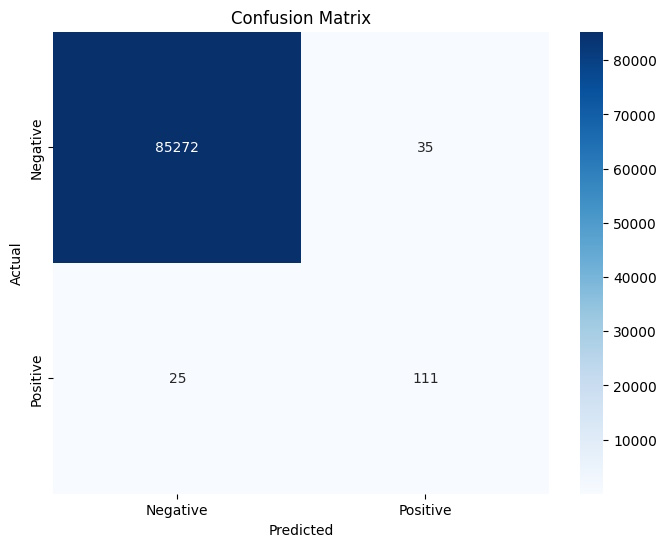
\includegraphics[width=0.8\linewidth]{images/confusion_matrix.jpg}
    \caption{Confusion Matrix of the Final Model}
    \label{fig:confusion-matrix}
\end{figure}

From this confusion matrix, we computed the following metrics:

\begin{itemize}
    \item \textbf{Precision}: The fraction of predicted fraudulent transactions that are correctly classified.
    \[
    \text{Precision} = \frac{TP}{TP + FP}
    \]

    \item \textbf{Recall} (Sensitivity): The fraction of actual fraudulent transactions correctly identified.
    \[
    \text{Recall} = \frac{TP}{TP + FN}
    \]

    \item \textbf{F1 Score}: The harmonic mean between Precision and Recall, providing a balanced metric.
    \[
    \text{F1 Score} = 2 \times \frac{\text{Precision} \times \text{Recall}}{\text{Precision} + \text{Recall}}
    \]

    \item \textbf{Accuracy}: The overall fraction of transactions correctly classified.
    \[
    \text{Accuracy} = \frac{TP + TN}{TP + TN + FP + FN}
    \]
\end{itemize}

The final classification results are summarized below:

\begin{itemize}
    \item Accuracy = $0.9993$
    \item Precision = $0.7603$
    \item Recall = $0.8162$
    \item Specificity = $0.9996$
    \item F1 Score = $0.7872$
\end{itemize}

These results demonstrate that our model effectively identifies fraudulent transactions while maintaining very high accuracy, highlighting its suitability for deployment in practical fraud detection scenarios.

\subsection{Discussion}
Our final classification model achieved strong performance metrics (Precision = $0.7603$, Recall = $0.8162$, F1-score = $0.7872$, Specificity = $0.9996$ and Accuracy = $0.9993$), demonstrating its capability to identify fraudulent transactions with a balanced combination of precision and recall. However, compared to the original results reported by Tayebi and El Kafhali~\cite{Tayebi2025} (Precision = $0.985$, Recall = $0.9705$, F1-score = $0.9777$, and Accuracy = $0.9999$), our model exhibited somewhat lower effectiveness in distinguishing fraudulent transactions, particularly in terms of precision and recall.

A key factor potentially contributing to this performance gap is our implementation of the autoencoder training phase. Specifically, the autoencoder's reconstruction quality for fraudulent transaction data was somewhat limited, resulting in synthetic samples with lower realism and variability. Consequently, the SVM filtering step discarded a significant portion of synthetic fraud samples, thereby restricting the size and diversity of our final training dataset. This limitation may have impacted the subsequent training and generalization capabilities of the ALSTM model.

To address this, future efforts could include enhancing the autoencoder's training procedure, such as experimenting with deeper architectures, varying the latent dimensions, or employing alternative regularization and data augmentation strategies. Such improvements may lead to higher-quality synthetic data generation and potentially bridge the observed performance discrepancy between our results and those of the original study.

\paragraph{Note on evaluation metrics computed in the original paper}
During the analysis of the model's performance, an inconsistency emerged concerning the definitions of evaluation metrics originally provided by the reference paper. Specifically, the definitions of \textbf{specificity} and \textbf{recall} were inverted compared to the commonly accepted standards in the literature. Using the formulas from the original paper, in our work, the newly computed specificity is $0.8162$ and recall is $0.9996$, resulting in an F1 Score of $0.8637$, which is significantly higher than the correct value of $0.7872$ obtained with standard definitions.

\section{Conclusion}
This project implemented a multi-stage fraud detection framework combining autoencoders, SVM filtering, and gradient-boosted ALSTM networks. Starting from a severely imbalanced dataset, we trained an autoencoder solely on fraudulent data to generate realistic synthetic fraud samples, refined them using an SVM classifier, and ultimately classified transactions with a powerful attention-based LSTM model within a gradient boosting ensemble.

Our results demonstrate the effectiveness of this approach in detecting rare fraudulent transactions with high accuracy and low false positive rates. The attention mechanism notably improved the model's ability to capture relevant temporal dependencies in sequential transaction data.



\balance

%%
%% The next two lines define the bibliography style to be used, and
%% the bibliography file.
\bibliographystyle{ACM-Reference-Format}
\interlinepenalty=10000
\bibliography{acmart}

\end{document}
\endinput
%%
%% End of file `sample-sigconf.tex'.
